\section{Results}
\label{sec:results}

\subsection{Controlled adaptive-refinement matrix}

The three refinement strategies were evaluated at four identical refinement
budgets, producing a controlled matrix of 12 adaptive CFD simulations.
Table~\ref{tab:adaptive_results} summarizes the principal results.

\begin{table}[htbp]
\centering
\caption{Adaptive-mesh results relative to the M160 fine-grid numerical
reference. Mean and RMS velocity discrepancies are volume weighted. CPU time
corresponds to the final CFD solve and does not include the complete adaptive
workflow cost.}
\label{tab:adaptive_results}
\small
\begin{tabular}{llrrrr}
\toprule
Method & Budget & Cells & CPU [s] & Mean error & RMS error \\
\midrule
Gradient & 5\%  & 1840 & 9.64  & 0.001846 & 0.003994 \\
Gradient & 10\% & 2080 & 11.64 & 0.001656 & 0.003756 \\
Gradient & 15\% & 2320 & 13.62 & 0.001296 & 0.003505 \\
Gradient & 20\% & 2560 & 14.05 & 0.001105 & 0.003384 \\
\midrule
SOM-QE & 5\%  & 1840 & 9.62  & 0.002349 & 0.004392 \\
SOM-QE & 10\% & 2080 & 11.24 & 0.002628 & 0.004492 \\
SOM-QE & 15\% & 2320 & 12.53 & 0.002291 & 0.004175 \\
SOM-QE & 20\% & 2560 & 13.77 & 0.002005 & 0.003924 \\
\midrule
Hybrid-v1 & 5\%  & 1840 & 9.32  & 0.001841 & 0.004031 \\
Hybrid-v1 & 10\% & 2080 & 11.09 & 0.001583 & 0.003709 \\
Hybrid-v1 & 15\% & 2320 & 12.50 & 0.001394 & 0.003556 \\
Hybrid-v1 & 20\% & 2560 & 14.68 & 0.001242 & 0.003453 \\
\bottomrule
\end{tabular}
\end{table}

All adaptive meshes passed the mesh-quality checks used in the automated
experiment framework. The maximum Courant number remained below the imposed
limit of 1.05 for all cases.

\subsection{RMS discrepancy}

Figure~\ref{fig:rms_cells} compares the volume-weighted RMS velocity
discrepancy as a function of final adaptive-mesh cell count.

\begin{figure}[htbp]
\centering
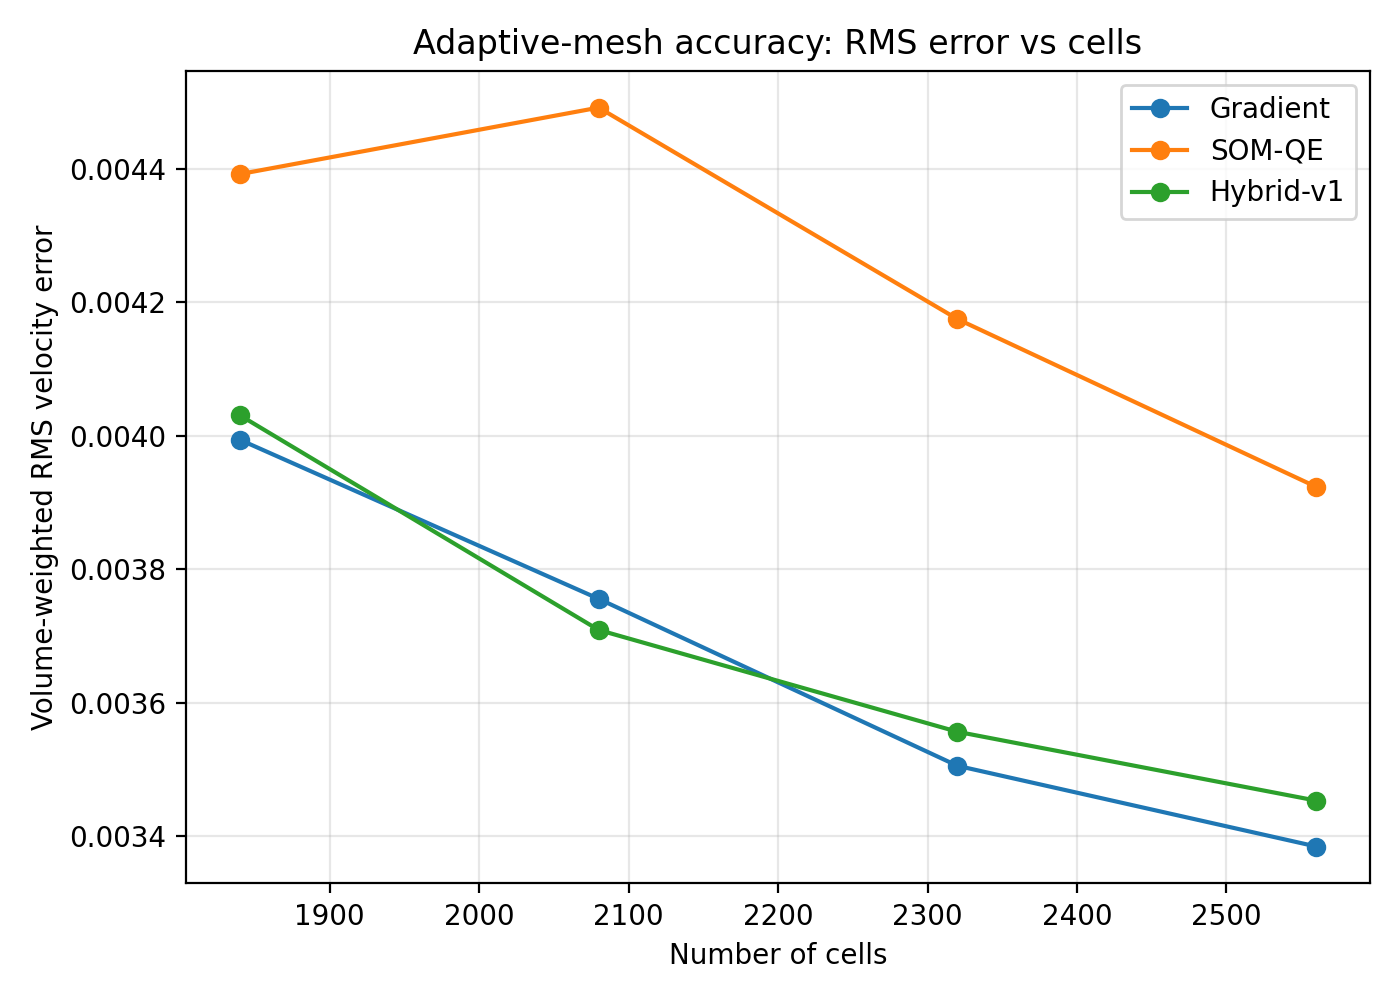
\includegraphics[width=0.88\textwidth]
{figures/RMS_vs_cells_3methods.png}
\caption{Volume-weighted RMS velocity discrepancy relative to the M160
fine-grid numerical reference for Gradient, SOM-QE, and Hybrid-v1 refinement.}
\label{fig:rms_cells}
\end{figure}

The Gradient criterion exhibits monotonic improvement as the refinement
budget increases. Its RMS discrepancy decreases from approximately
\(3.994\times10^{-3}\) at the 5\% budget to
\(3.384\times10^{-3}\) at the 20\% budget.

Direct SOM-QE refinement does not exhibit the same behavior. In particular,
increasing the budget from 5\% to 10\% increases the RMS discrepancy from

\begin{equation}
4.392\times10^{-3}
\end{equation}

to

\begin{equation}
4.492\times10^{-3}.
\end{equation}

The SOM-QE criterion subsequently improves at the 15\% and 20\% budgets, but
its RMS discrepancy remains higher than that of Gradient at every tested
budget.

At equal refinement budgets, the Gradient RMS discrepancy is lower than the
SOM-QE result by approximately 9.1\%, 16.4\%, 16.0\%, and 13.7\% for the
5\%, 10\%, 15\%, and 20\% budgets, respectively.

These results do not support the hypothesis that SOM quantization error can
be used directly as a superior refinement indicator for the present cavity
problem.

\subsection{Hybrid-v1 performance}

Hybrid-v1 recovers monotonic RMS improvement with increasing refinement
budget and remains close to the Gradient baseline.

Relative to Gradient, the Hybrid-v1 RMS discrepancy changes by approximately

\begin{equation}
-0.92\%,\quad
+1.24\%,\quad
-1.45\%,\quad
-2.03\%
\end{equation}

at the 5\%, 10\%, 15\%, and 20\% budgets, respectively, where a positive
value denotes an improvement relative to Gradient.

Thus, Hybrid-v1 produces a small RMS improvement at the 10\% budget, but this
improvement is not reproduced at the other tested budgets. The present
results therefore do not demonstrate a systematic accuracy advantage of
Hybrid-v1 over the conventional Gradient criterion.

\subsection{Mean velocity discrepancy}

Figure~\ref{fig:mean_cells} presents the corresponding volume-weighted mean
velocity discrepancy.

\begin{figure}[htbp]
\centering
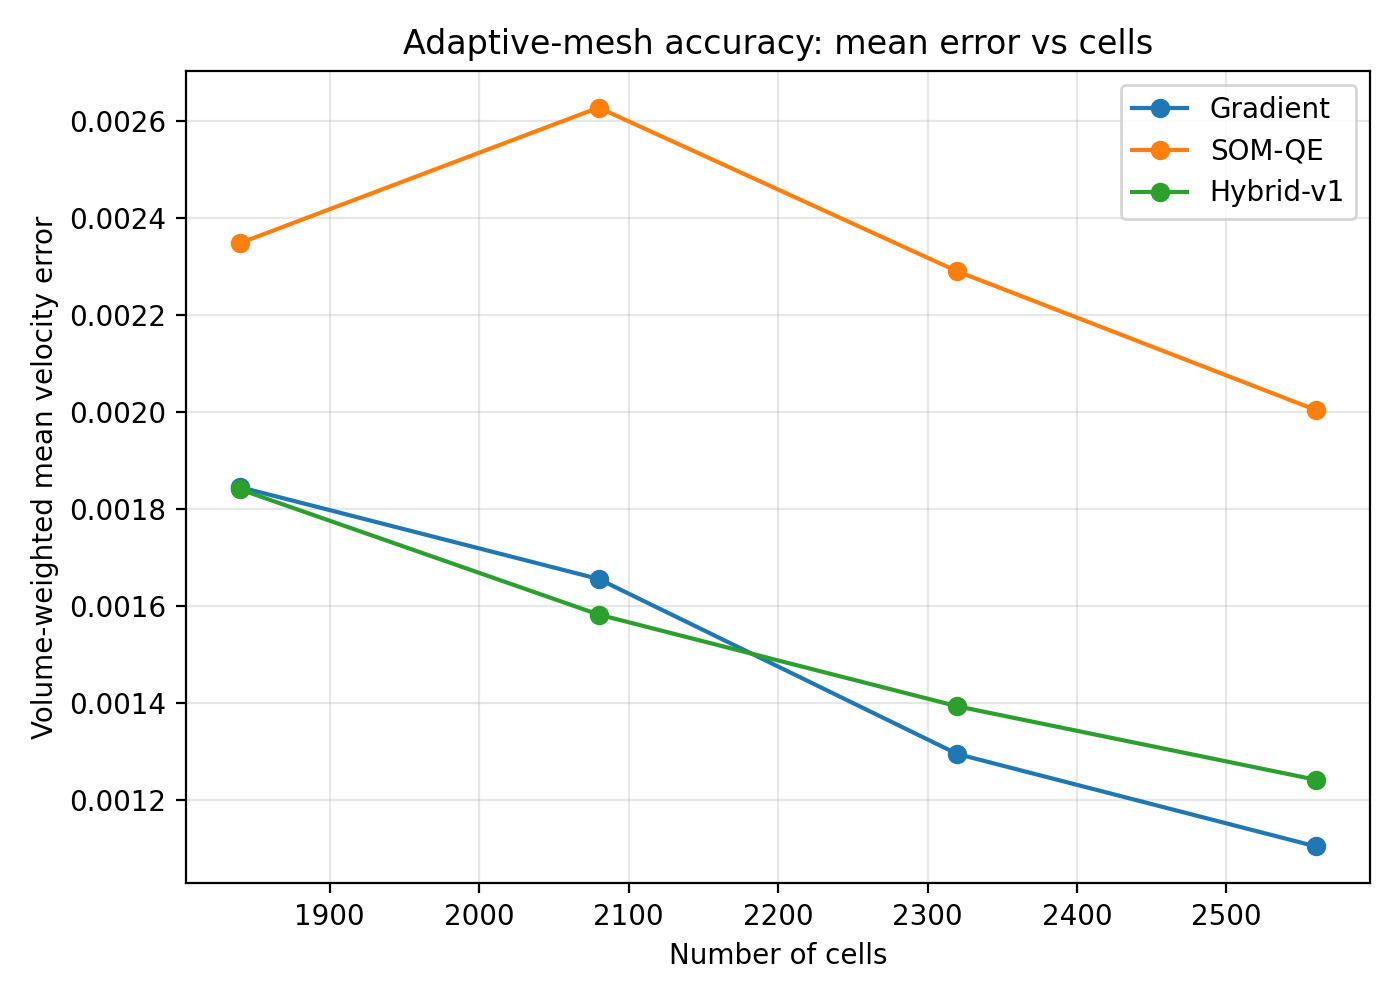
\includegraphics[width=0.88\textwidth]
{figures/Mean_vs_cells_3methods.png}
\caption{Volume-weighted mean velocity discrepancy relative to the M160
fine-grid numerical reference for the three refinement strategies.}
\label{fig:mean_cells}
\end{figure}

The mean-error results reinforce the RMS comparison. Gradient improves
monotonically from approximately \(1.846\times10^{-3}\) to
\(1.105\times10^{-3}\).

SOM-QE again exhibits non-monotonic behavior between the 5\% and 10\%
budgets. At the four tested budgets, the Gradient mean discrepancy is
approximately 21.4\%, 37.0\%, 43.4\%, and 44.9\% lower than the corresponding
SOM-QE result.

Hybrid-v1 produces a mean-error improvement of approximately 0.25\% and
4.43\% relative to Gradient at the 5\% and 10\% budgets, respectively.
However, at 15\% and 20\% its mean discrepancy is approximately 7.59\% and
12.44\% higher than Gradient.

As with the RMS metric, the hybrid modification therefore does not provide a
consistent advantage across refinement budgets.

\subsection{What Hybrid-v1 changes}

Because Hybrid-v1 preserves the gradient as its primary signal, its cell
selection remains strongly overlapping with the conventional Gradient
selection.

Figure~\ref{fig:gradient_hybrid_selection} shows the spatial distribution of
common and exclusive selections at all four budgets.

\begin{figure}[htbp]
\centering
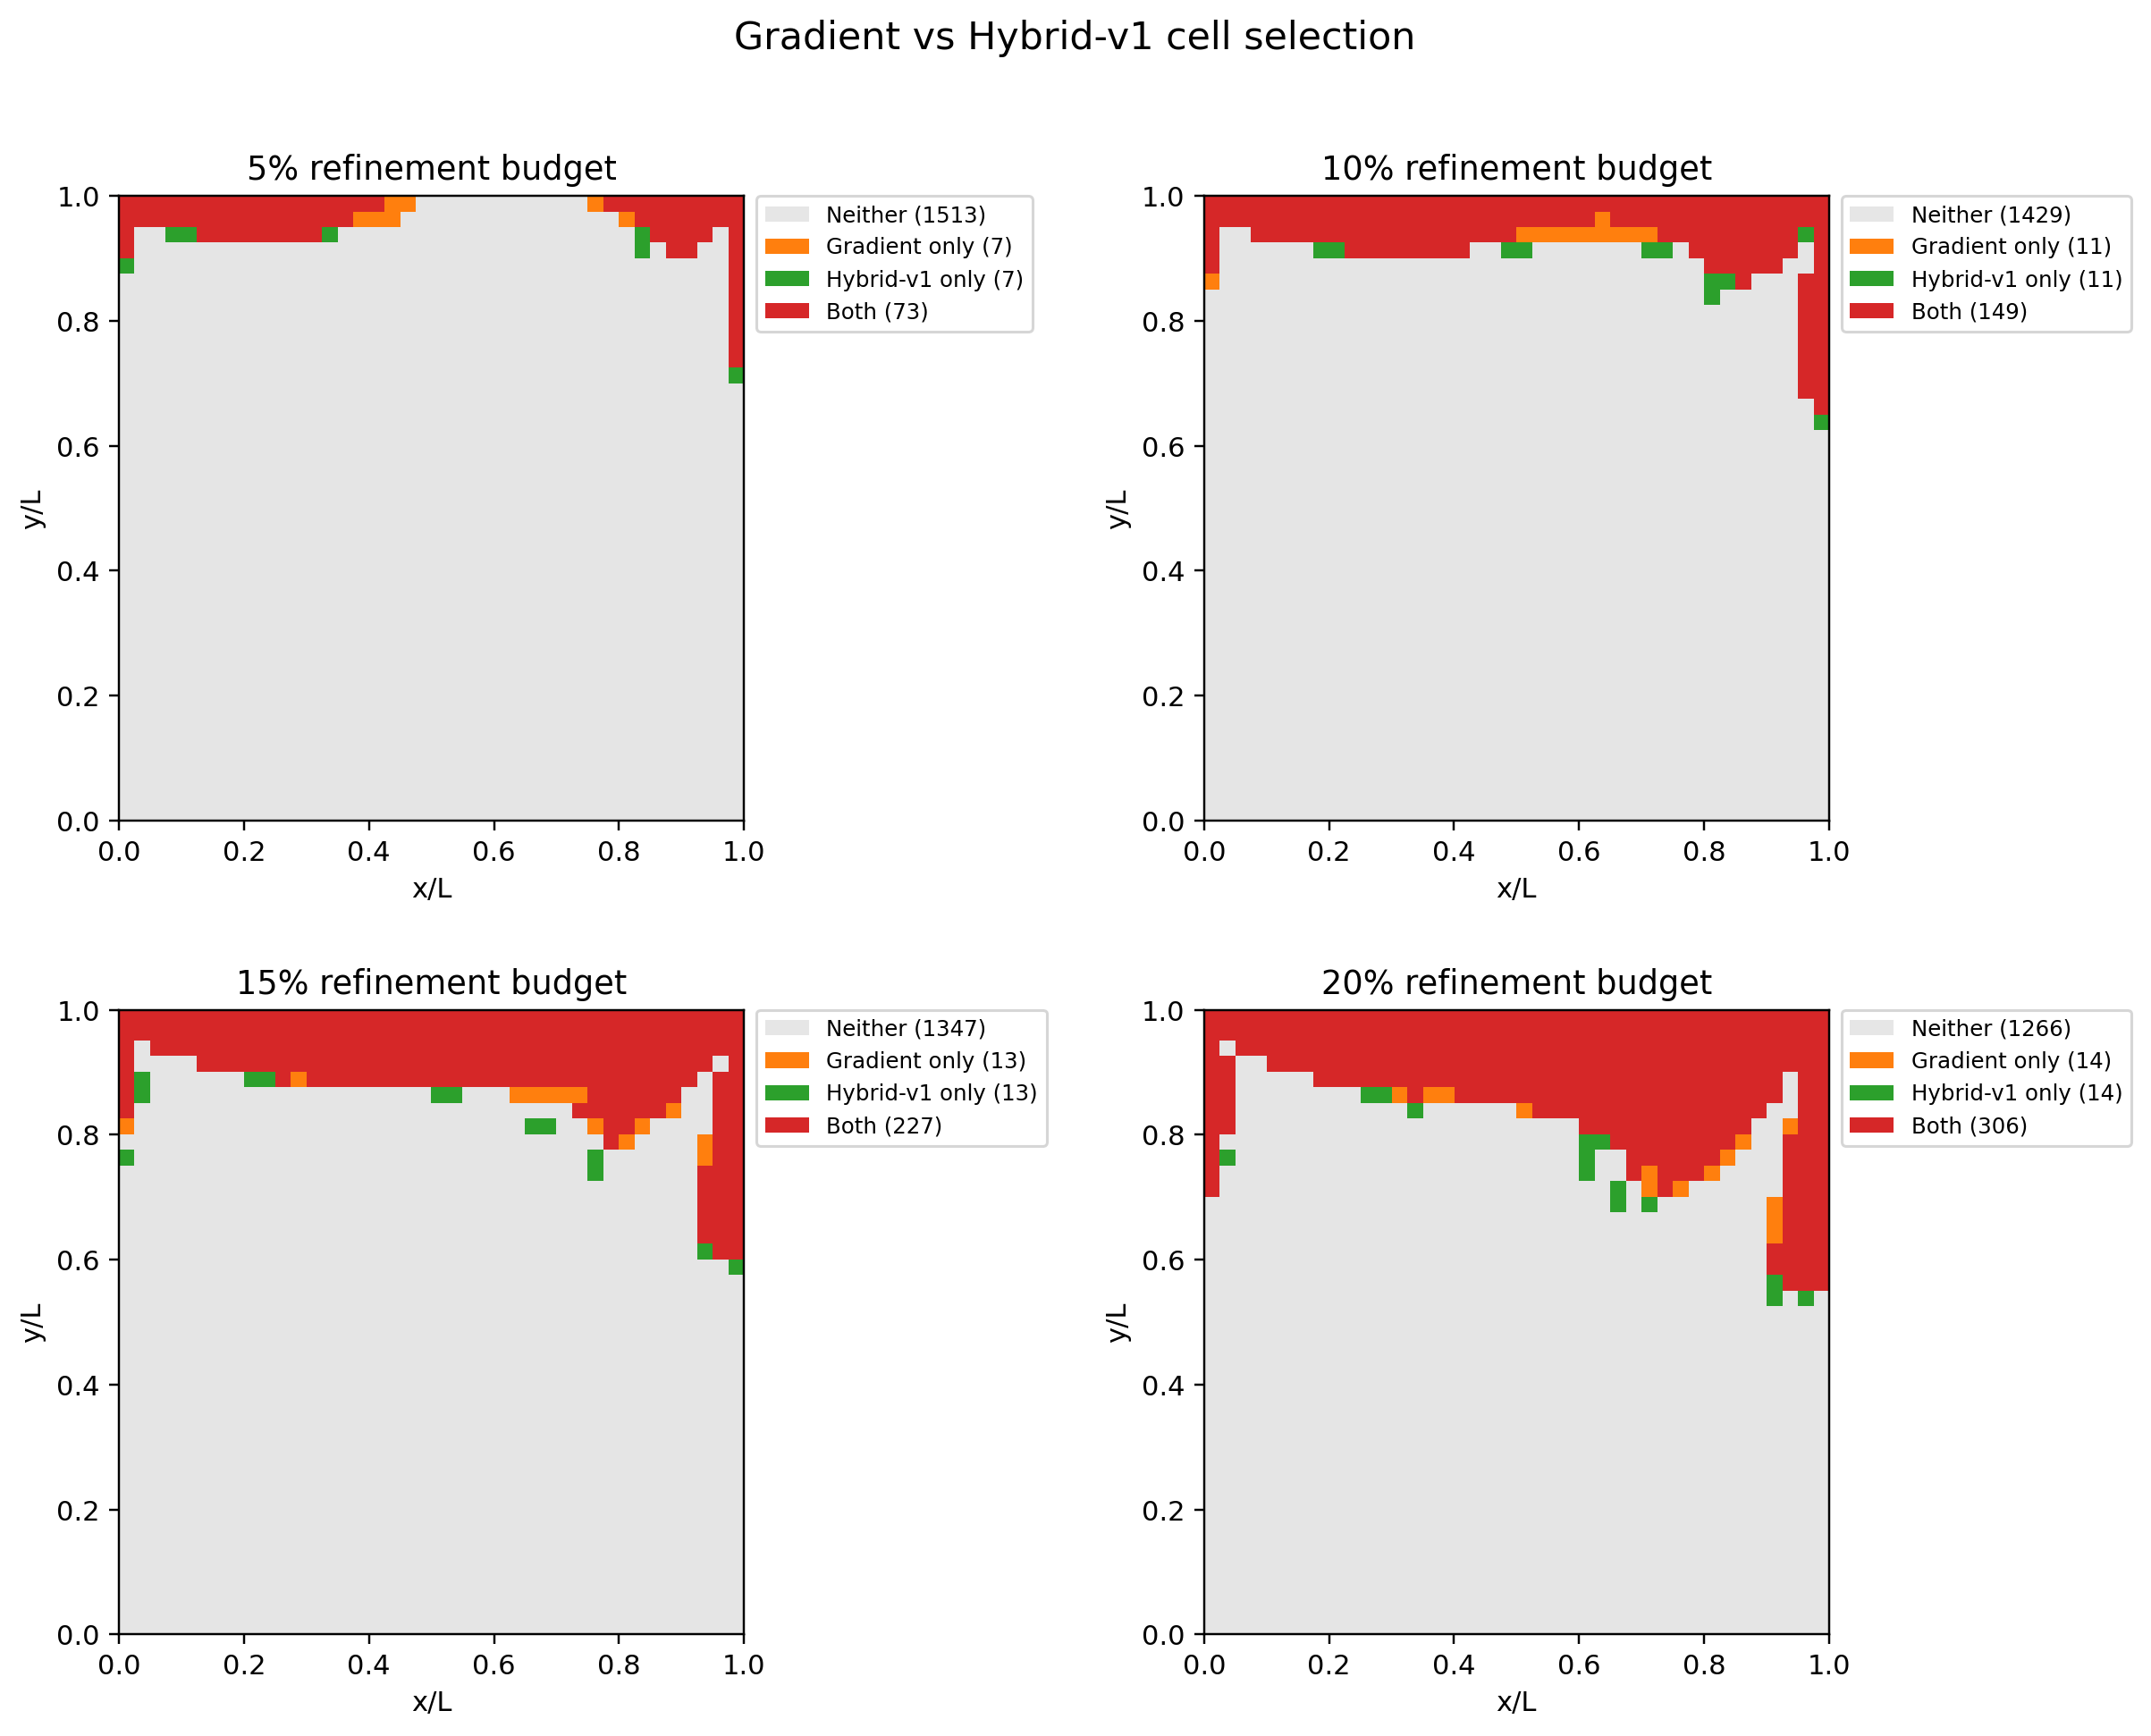
\includegraphics[width=0.98\textwidth]
{figures/Gradient_vs_Hybrid_selection_all_budgets.png}
\caption{Comparison of Gradient and Hybrid-v1 cell selections for refinement
budgets of 5\%, 10\%, 15\%, and 20\%. The hybrid formulation changes only a
small subset of cells close to the selection threshold.}
\label{fig:gradient_hybrid_selection}
\end{figure}

The overlap increases from 91.25\% at the 5\% budget to 95.62\% at the
20\% budget. Hybrid-v1 therefore acts as a controlled modification of the
Gradient ranking rather than as an independent replacement criterion.

To identify the physical nature of these changes, the cells selected
exclusively by each method were analyzed using only quantities available from
the M40 pilot solution. Table~\ref{tab:swap_statistics} summarizes the
results.

\begin{table}[htbp]
\centering
\caption{Mean characteristics of cells selected exclusively by Gradient or
Hybrid-v1. The analysis uses only M40 quantities and does not use the M160
reference.}
\label{tab:swap_statistics}
\small
\begin{tabular}{llrrr}
\toprule
Budget & Exclusive selection & Cells &
Mean $|\nabla U|^{*}$ & Mean $T$ \\
\midrule
5\%  & Gradient  & 7  & 7.489 & 0.000 \\
5\%  & Hybrid-v1 & 7  & 6.663 & 0.619 \\
10\% & Gradient  & 11 & 5.384 & 0.000 \\
10\% & Hybrid-v1 & 11 & 4.810 & 0.583 \\
15\% & Gradient  & 13 & 3.730 & 0.000 \\
15\% & Hybrid-v1 & 13 & 3.261 & 0.596 \\
20\% & Gradient  & 14 & 2.836 & 0.054 \\
20\% & Hybrid-v1 & 14 & 2.461 & 0.643 \\
\bottomrule
\end{tabular}
\end{table}

A consistent pattern is observed at all four budgets. Hybrid-v1 removes a
small number of cells having somewhat larger velocity gradients but little or
no SOM regime-transition activity and replaces them with cells having
slightly smaller gradients but substantially larger transition indicators.

For example, at the 10\% budget the Gradient-only cells have mean values

\begin{equation}
|\nabla U|^{*}=5.384,
\qquad
T=0,
\end{equation}

whereas the Hybrid-only cells have

\begin{equation}
|\nabla U|^{*}=4.810,
\qquad
T=0.583.
\end{equation}

The hybrid formulation is therefore behaving according to its intended
design: SOM information changes the priority of cells located near boundaries
between SOM-classified flow regimes.

However, the adaptive CFD results demonstrate that this physically
interpretable modification is not systematically beneficial. The 10\% case
improves the RMS discrepancy, whereas the same mechanism slightly worsens the
RMS result at 5\%, 15\%, and 20\%.

This distinction motivates a central result of the present investigation:
information that identifies a physically distinct flow state or a boundary
between states is not necessarily equivalent to information that predicts
the numerical utility of refining that location.

\subsection{Computational-time observations}

The measured solver execution times increase with final cell count, as
expected. Differences between methods at equal cell count are relatively
small compared with the differences in accuracy.

No claim of computational-speed superiority is made from these measurements.
Only one timing measurement was collected for each case, and the reported
solver times exclude the cost of pilot CFD calculation, SOM training,
indicator construction, mesh refinement, field mapping, and other workflow
operations.

A rigorous computational-efficiency comparison would require repeated timing
measurements and accounting for the complete adaptive workflow.



\subsection{Second-stage SOM-interface experiments}

The preceding results motivated a change in the SOM evaluation criterion.
Direct quantization error was not treated as a discretization-error
estimator. Instead, the SOM classification was used to identify interfaces
between distinct local flow states, and these interfaces were ranked using
the indicator

\begin{equation}
I_{\mathrm{SI}}
=
T\sqrt{G^*\Delta U^*}.
\end{equation}

A fixed set of 40 highest-ranked interface seeds was used for both
experiments. The refinement region was then expanded by one graph layer
(\(1N\)) or two graph layers (\(2N\)). The two cases selected 78 and 114
M40 parent cells, respectively, producing final meshes with 1834 and 1942
cells.

\begin{table}[htbp]
\centering
\caption{SOM-interface experiments and cell-matched Gradient controls. The
Gradient cases use exactly the same number of selected M40 parent cells and
therefore produce the same final cell counts.}
\label{tab:som_interface_matched}
\small
\begin{tabular}{lrrrrrr}
\toprule
Case & Method & Seeds & Selected & Cells & Mean error & RMS error \\
\midrule
1N & SOM-interface & 40 & 78  & 1834 & 0.001570 & 0.003929 \\
1N & Gradient      & -- & 78  & 1834 & 0.001824 & 0.003986 \\
2N & SOM-interface & 40 & 114 & 1942 & 0.001359 & 0.003611 \\
2N & Gradient      & -- & 114 & 1942 & 0.001672 & 0.003761 \\
\bottomrule
\end{tabular}
\end{table}

All four cell-matched experiments completed successfully to \(t=5\).
The maximum Courant numbers were 0.926 for SOM-interface \(1N\), 0.930 for
SOM-interface \(2N\), 0.952 for Gradient-78, and 0.961 for Gradient-114,
remaining below the imposed limit of 1.05.

At 1834 cells, the SOM-interface case reduced the volume-weighted mean
velocity discrepancy by approximately \(13.9\%\) relative to the
cell-matched Gradient case. The RMS discrepancy was reduced by approximately
\(1.4\%\).

At 1942 cells, the corresponding reductions were approximately \(18.7\%\)
for the mean discrepancy and \(4.0\%\) for the RMS discrepancy.

The maximum pointwise discrepancy remained very similar for the paired
cases and occurred at the same normalized upper-corner location. For the
\(1N\) pair, the SOM-interface maximum was \(0.136204\), compared with
\(0.136135\) for Gradient. For the \(2N\) pair, the corresponding values
were \(0.136151\) and \(0.136135\). Thus, the observed improvement is
primarily reflected in the volume-weighted global metrics rather than in the
maximum pointwise discrepancy.

\begin{figure}[htbp]
\centering
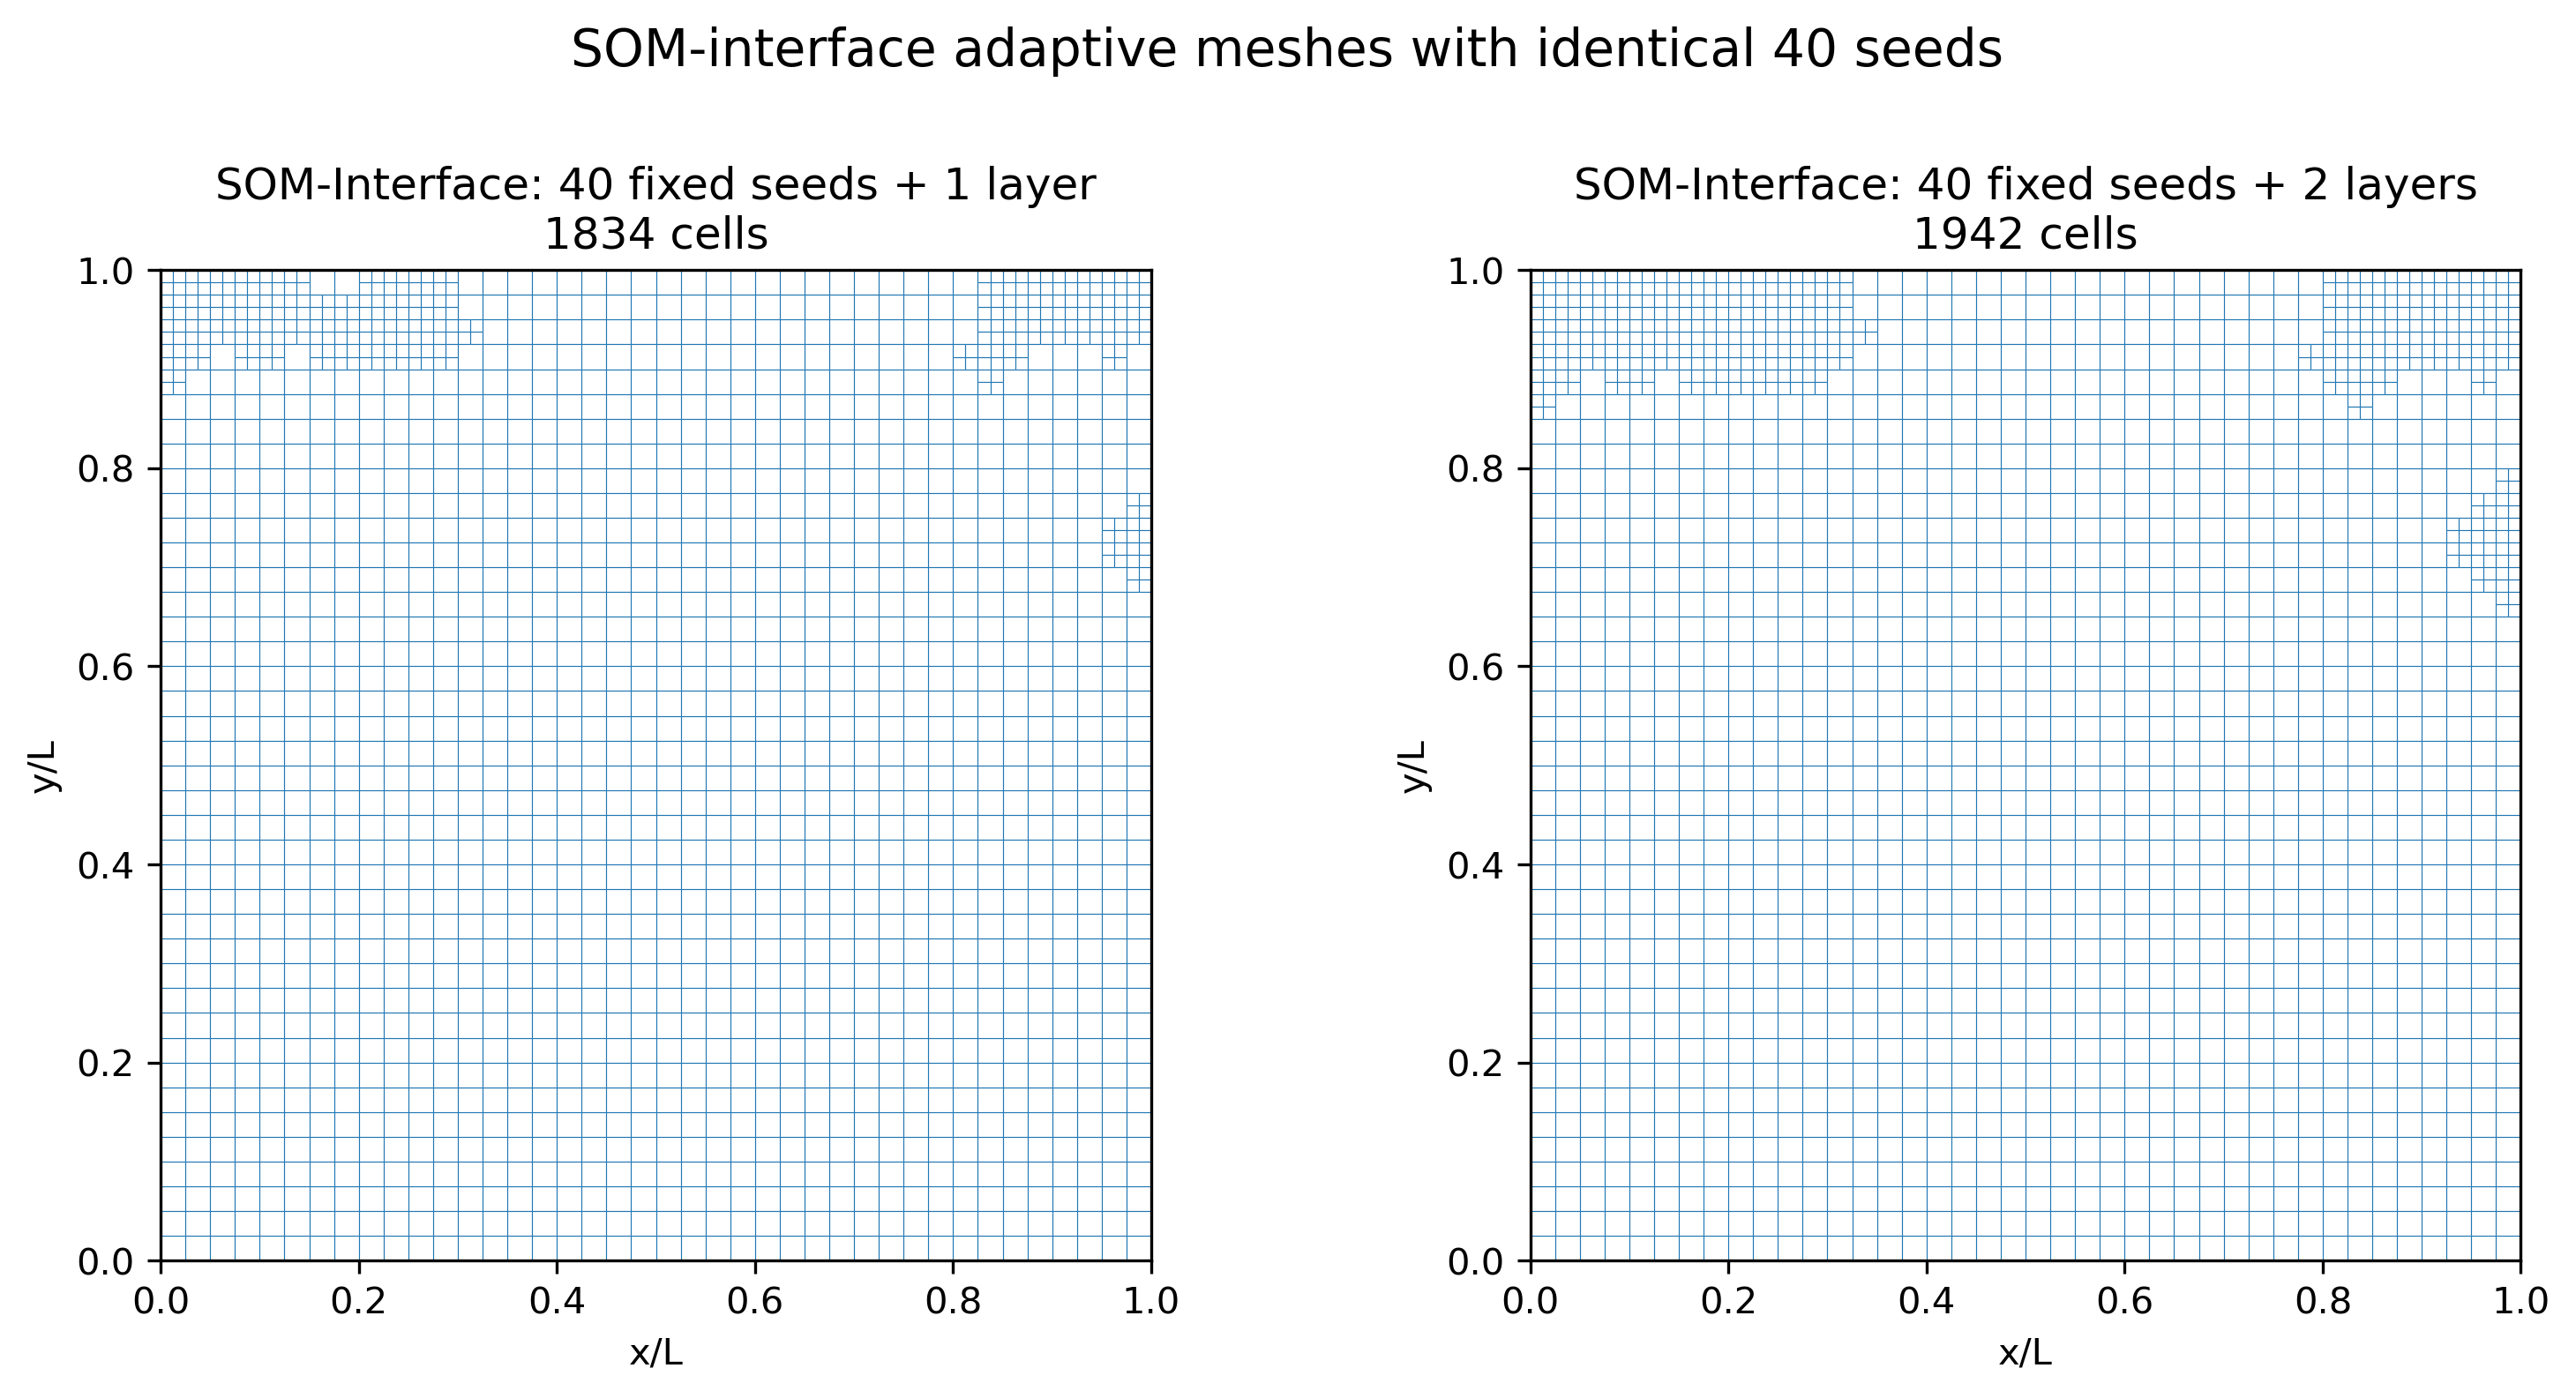
\includegraphics[width=0.92\textwidth]
{figures/SOM_Interface_real_mesh_1N_vs_2N.png}
\caption{Final adaptive meshes produced by the SOM-interface criterion using
the same 40 frozen interface seeds and one or two graph layers. The cases
contain 1834 and 1942 cells, respectively.}
\label{fig:som_interface_real_meshes}
\end{figure}

The real-mesh comparison shows that the second-stage criterion does not
simply refine isolated high-gradient cells. Instead, the fixed interface
seeds generate spatially connected refinement regions. Increasing the graph
radius from one to two layers preserves the same seed set and adds 36
additional cells, increasing the final mesh from 1834 to 1942 cells.

\begin{figure}[htbp]
\centering
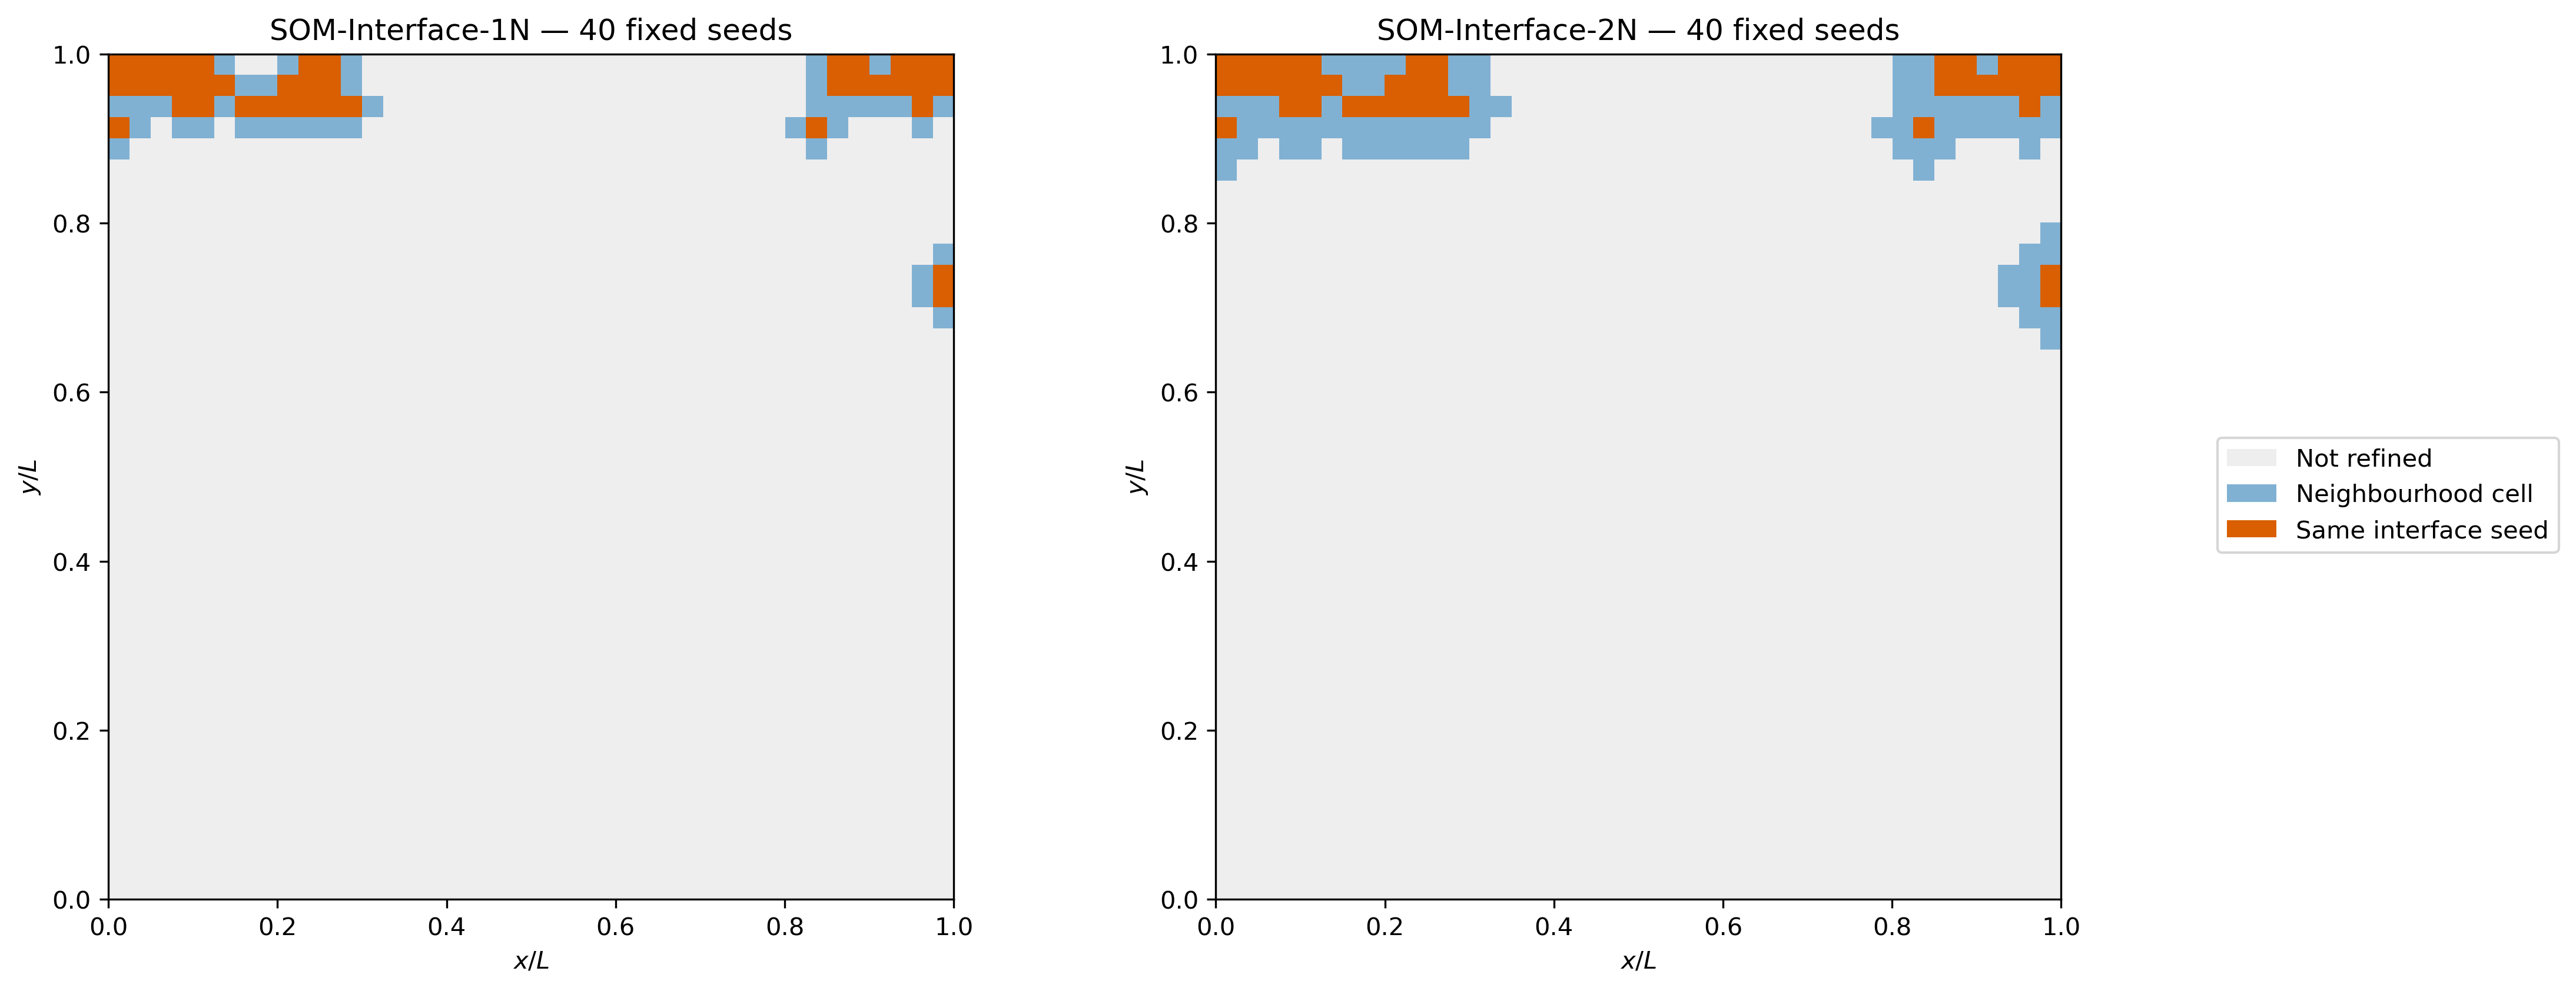
\includegraphics[width=0.88\textwidth]
{figures/SOM_Interface_fixed_seeds_1N_vs_2N.png}
\caption{Selection obtained from the same 40 frozen SOM-interface seeds for
one and two graph-layer expansions. The \(1N\) selection is a subset of the
\(2N\) selection; the latter adds 36 cells.}
\label{fig:som_interface_fixed_seeds}
\end{figure}

\subsection{Gradient versus SOM-interface selection overlap}

The cell-matched comparisons also show that the new criterion is related to,
but not identical with, the conventional Gradient criterion. For the
1834-cell comparison, 53 of the 78 selected cells were common to both
methods, corresponding to an overlap of \(67.95\%\). Each method selected
25 additional cells not selected by the other.

For the 1942-cell comparison, 74 of the 114 selected cells were common,
corresponding to an overlap of \(64.91\%\). Gradient selected 40 cells that
were not selected by SOM-interface, while SOM-interface selected another
40 cells.

\begin{figure}[htbp]
\centering
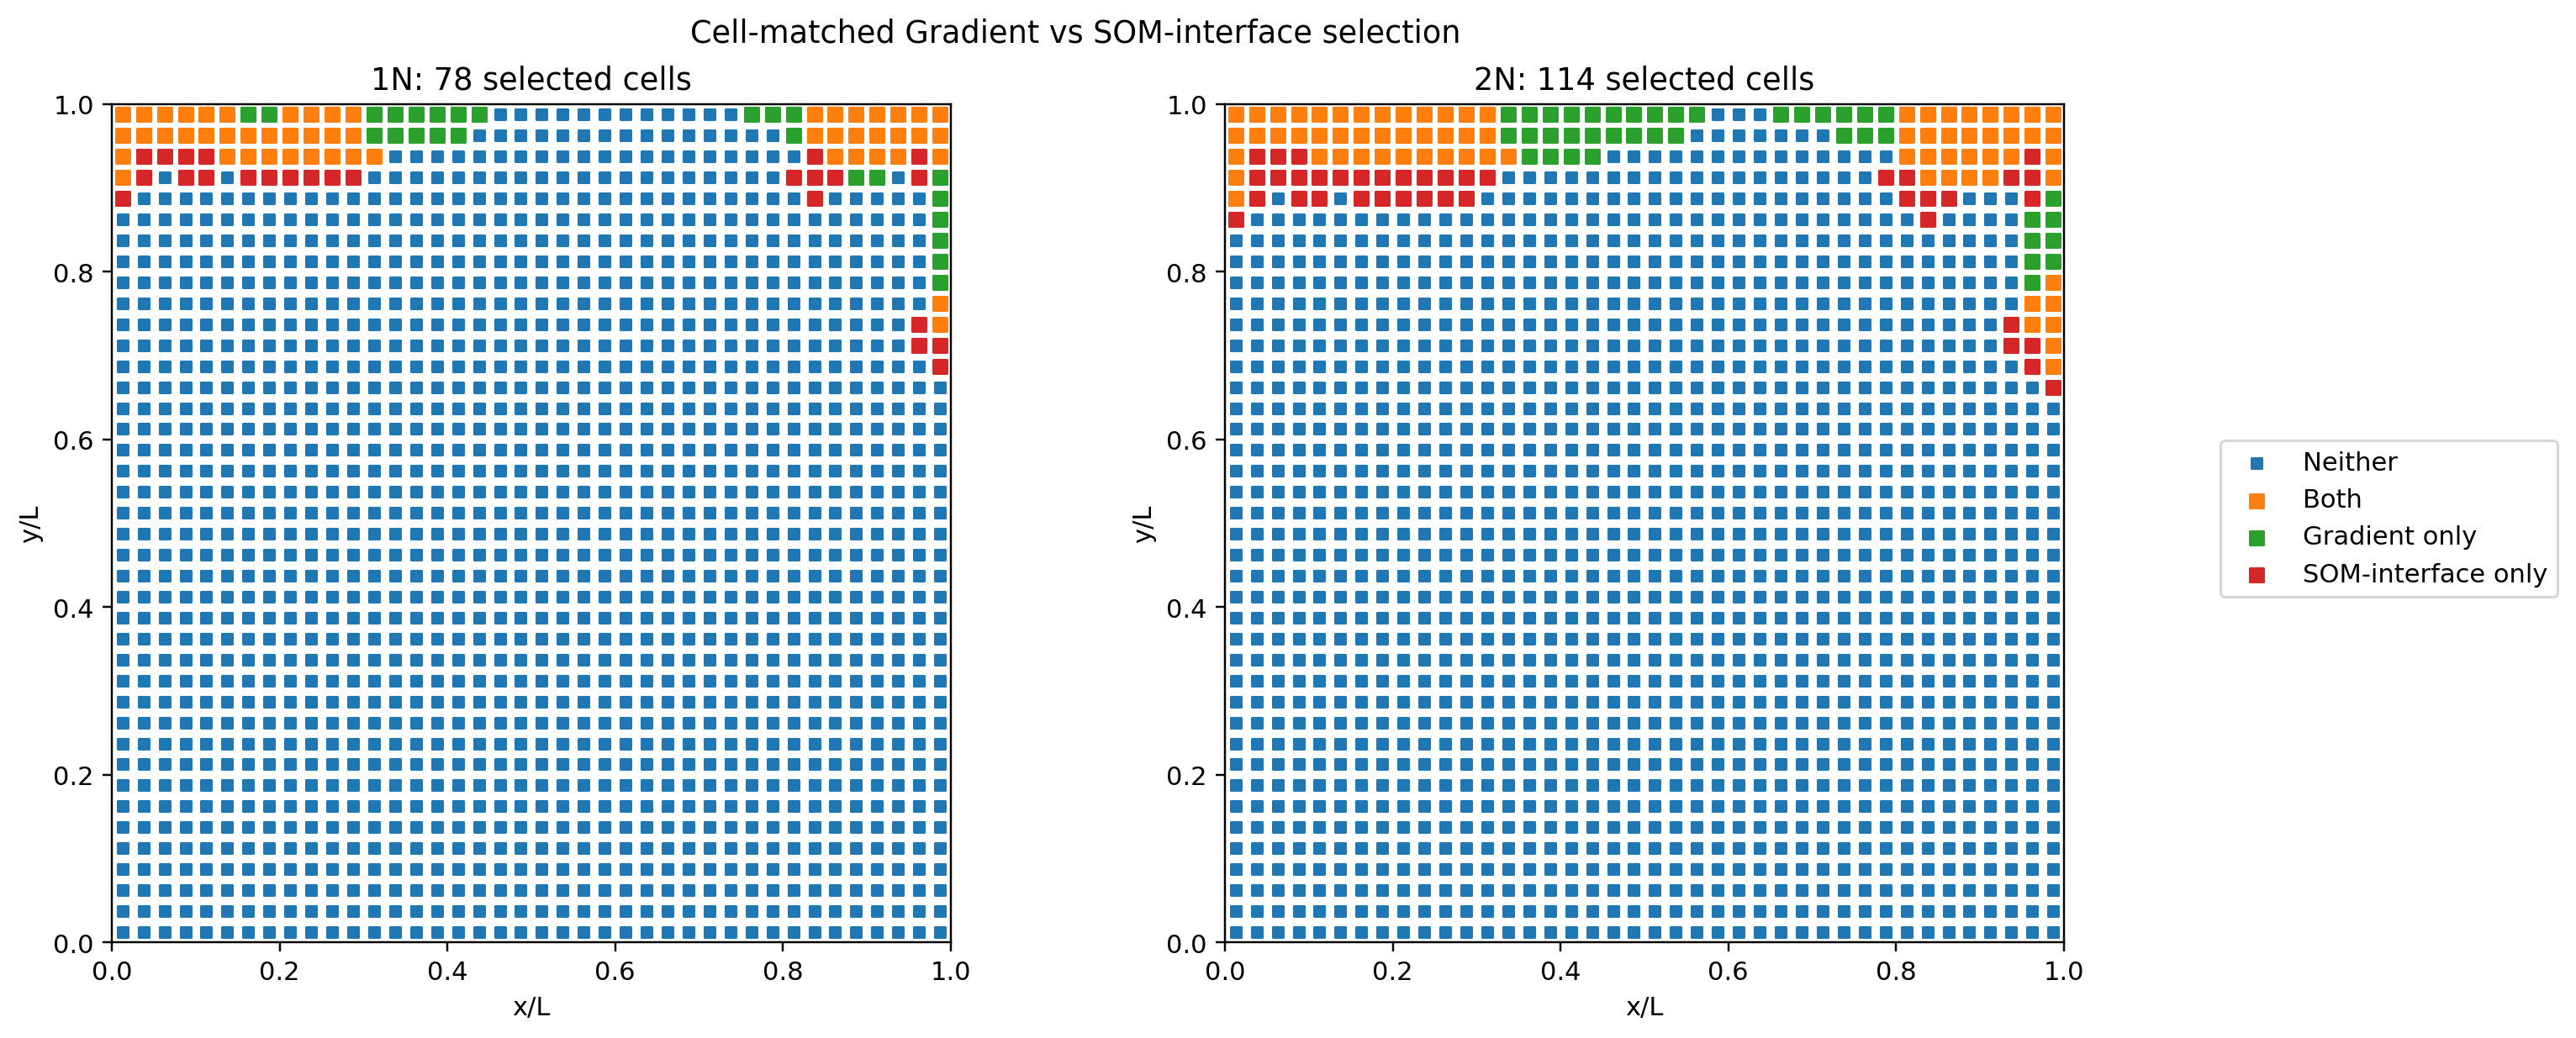
\includegraphics[width=0.90\textwidth]
{figures/Gradient_vs_SOM_Interface_cell_matched.png}
\caption{Cell-by-cell comparison between Gradient and SOM-interface
selections at matched final mesh sizes. The methods share a substantial
fraction of selected cells while allocating the remaining refinement budget
differently.}
\label{fig:gradient_som_interface_overlap}
\end{figure}

These overlaps are important because the new results cannot be explained by
a completely different refinement philosophy. A substantial portion of the
selected cells is common to both methods. The numerical differences arise
from the spatial allocation of the remaining refinement cells.

\subsection{SOM Architecture and Initialization Sensitivity}
\label{sec:som_sensitivity}

A sensitivity study was performed to determine how the SOM representation
depends on lattice architecture and random initialization. Four square
architectures were evaluated: \(3\times3\), \(4\times4\), \(5\times5\),
and \(6\times6\), corresponding to 9, 16, 25, and 36 neurons,
respectively.

For each architecture, five independent initializations were evaluated using
random seeds 1, 11, 21, 31, and 42, giving a total of 20 SOM training runs.
The M40 CFD solution, input features, feature standardization, SOM training
algorithm, and 20000 training iterations were held fixed across all runs.
The initial neighborhood width was also kept fixed at
\(\sigma_0=2\). Consequently, its size relative to the SOM lattice changes
with architecture; this choice was retained deliberately so that the tested
configurations differed only in lattice size and random initialization under
the common training specification.

The sensitivity analysis considered several complementary quantities:
quantization error, SOM-interface fraction, partition stability between
random initializations, and spatial stability of the 40 highest-priority
interface seeds. These metrics characterize different properties of the SOM
and should not individually be interpreted as measures of adaptive-mesh
accuracy.

Table~\ref{tab:som_architecture_sensitivity} summarizes the architecture-level
statistics obtained by averaging over the five random initializations.

\begin{table}[htbp]
\centering
\caption{Sensitivity of the SOM representation to lattice architecture.
Reported values are averages over five random seeds.}
\label{tab:som_architecture_sensitivity}
\begin{tabular}{cccccc}
\hline
Architecture & Neurons & Mean QE & SD QE & Interface fraction & Occupied neurons \\
\hline
\(3\times3\) & 9  & 0.6468 & 0.0136 & 0.3078 & 9.0 \\
\(4\times4\) & 16 & 0.5049 & 0.0166 & 0.4381 & 16.0 \\
\(5\times5\) & 25 & 0.4023 & 0.0036 & 0.5478 & 25.0 \\
\(6\times6\) & 36 & 0.3431 & 0.0037 & 0.6304 & 35.8 \\
\hline
\end{tabular}
\end{table}

Increasing the number of SOM neurons systematically reduced the mean
quantization error for the tested configurations. The mean QE decreased from
approximately 0.647 for the \(3\times3\) architecture to 0.343 for the
\(6\times6\) architecture. This behavior is expected because a larger number
of prototypes provides greater representational capacity in the standardized
feature space.

At the same time, the fraction of M40 cells classified as SOM-interface cells
increased substantially, from approximately 30.8\% for \(3\times3\) to
43.8\% for \(4\times4\), 54.8\% for \(5\times5\), and 63.0\% for
\(6\times6\). Thus, increasing SOM resolution produces a finer partition of
the CFD state space but also generates a progressively denser spatial
interface network.

The reduction in quantization error should therefore not be interpreted as
evidence that the larger SOM architectures are automatically preferable for
adaptive refinement. Quantization error measures representation in feature
space, whereas the usefulness of a SOM-derived refinement criterion depends
on how the resulting state partition and interfaces contribute to subsequent
mesh-refinement decisions.

\subsubsection{Partition stability across random initializations}

Because SOM training depends on initialization, the stability of the learned
cell partition was evaluated across the five random seeds. Direct comparison
of BMU labels is not sufficient because neuron labels can be permuted between
independent SOM trainings. Partition similarity was therefore evaluated using
the Adjusted Rand Index (ARI) and a same-cluster pairwise Jaccard measure.

\begin{table}[htbp]
\centering
\caption{Stability of the SOM partition across random initializations.
Statistics are calculated from pairwise comparisons between the five seeds
for each architecture.}
\label{tab:som_partition_stability}
\begin{tabular}{ccccc}
\hline
Architecture & Mean ARI & SD ARI & Mean pair Jaccard & SD pair Jaccard \\
\hline
\(3\times3\) & 0.901 & 0.021 & 0.847 & 0.029 \\
\(4\times4\) & 0.771 & 0.031 & 0.656 & 0.038 \\
\(5\times5\) & 0.795 & 0.043 & 0.679 & 0.058 \\
\(6\times6\) & 0.674 & 0.051 & 0.526 & 0.056 \\
\hline
\end{tabular}
\end{table}

The \(3\times3\) architecture produced the most stable partition among the
tested configurations, with a mean ARI of approximately 0.901. The
\(6\times6\) architecture produced the lowest mean ARI, approximately 0.674.
The behavior was not strictly monotonic with lattice size: the \(5\times5\)
architecture was somewhat more stable than the \(4\times4\) architecture
according to both partition metrics.

These results show that the reduction in quantization error obtained with
larger maps does not imply increased robustness to random initialization.
In particular, the \(6\times6\) configuration achieved the lowest mean
quantization error while also exhibiting the lowest partition stability of
the four architectures tested. Architecture selection therefore involves
more than minimizing quantization error alone.

\subsubsection{Spatial stability of high-priority interface seeds}

Partition stability does not by itself determine whether the cells considered
most important for refinement move to completely different physical regions.
The spatial stability of the 40 highest-priority SOM-interface seeds was
therefore evaluated separately.

\begin{table}[htbp]
\centering
\caption{Spatial stability of the 40 highest-priority SOM-interface seeds
across random initializations.}
\label{tab:som_spatial_stability}
\begin{tabular}{ccccc}
\hline
Architecture & Exact Jaccard & Exact match & \(r=1\) match & \(r=2\) match \\
\hline
\(3\times3\) & 0.698 & 0.820 & 0.955 & 0.986 \\
\(4\times4\) & 0.507 & 0.665 & 0.895 & 0.960 \\
\(5\times5\) & 0.551 & 0.708 & 0.931 & 0.970 \\
\(6\times6\) & 0.609 & 0.753 & 0.951 & 0.988 \\
\hline
\end{tabular}
\end{table}

Exact agreement between the Top-40 seed sets varied appreciably with random
initialization. For the \(4\times4\) architecture used in the main study,
the mean exact Jaccard similarity was approximately 0.507 and the mean exact
cell-match fraction was 0.665.

However, much of this variation was spatially local. When a selected cell
was considered matched if a corresponding selection occurred within one
M40 cell layer, the mean match fraction for the \(4\times4\) architecture
increased to approximately 0.895. With a two-cell-layer tolerance it
increased to approximately 0.960. Similar behavior was observed for the
other tested architectures.

These proximity statistics indicate that different initializations often
identify nearby regions even when they do not select exactly the same cells.
They should nevertheless be interpreted cautiously: the proximity measure
allows local many-to-one correspondence and is not equivalent to the overlap
of the final refined regions or to equality of the resulting adaptive CFD
solutions.

Figure~\ref{fig:som_sensitivity_consensus} provides a spatial view of these
sensitivity results. The upper row shows how frequently each M40 cell was
classified as a SOM-interface cell across the five random initializations,
whereas the lower row shows the corresponding selection frequency among the
40 highest-priority interface seeds.

\begin{figure}[htbp]
\centering
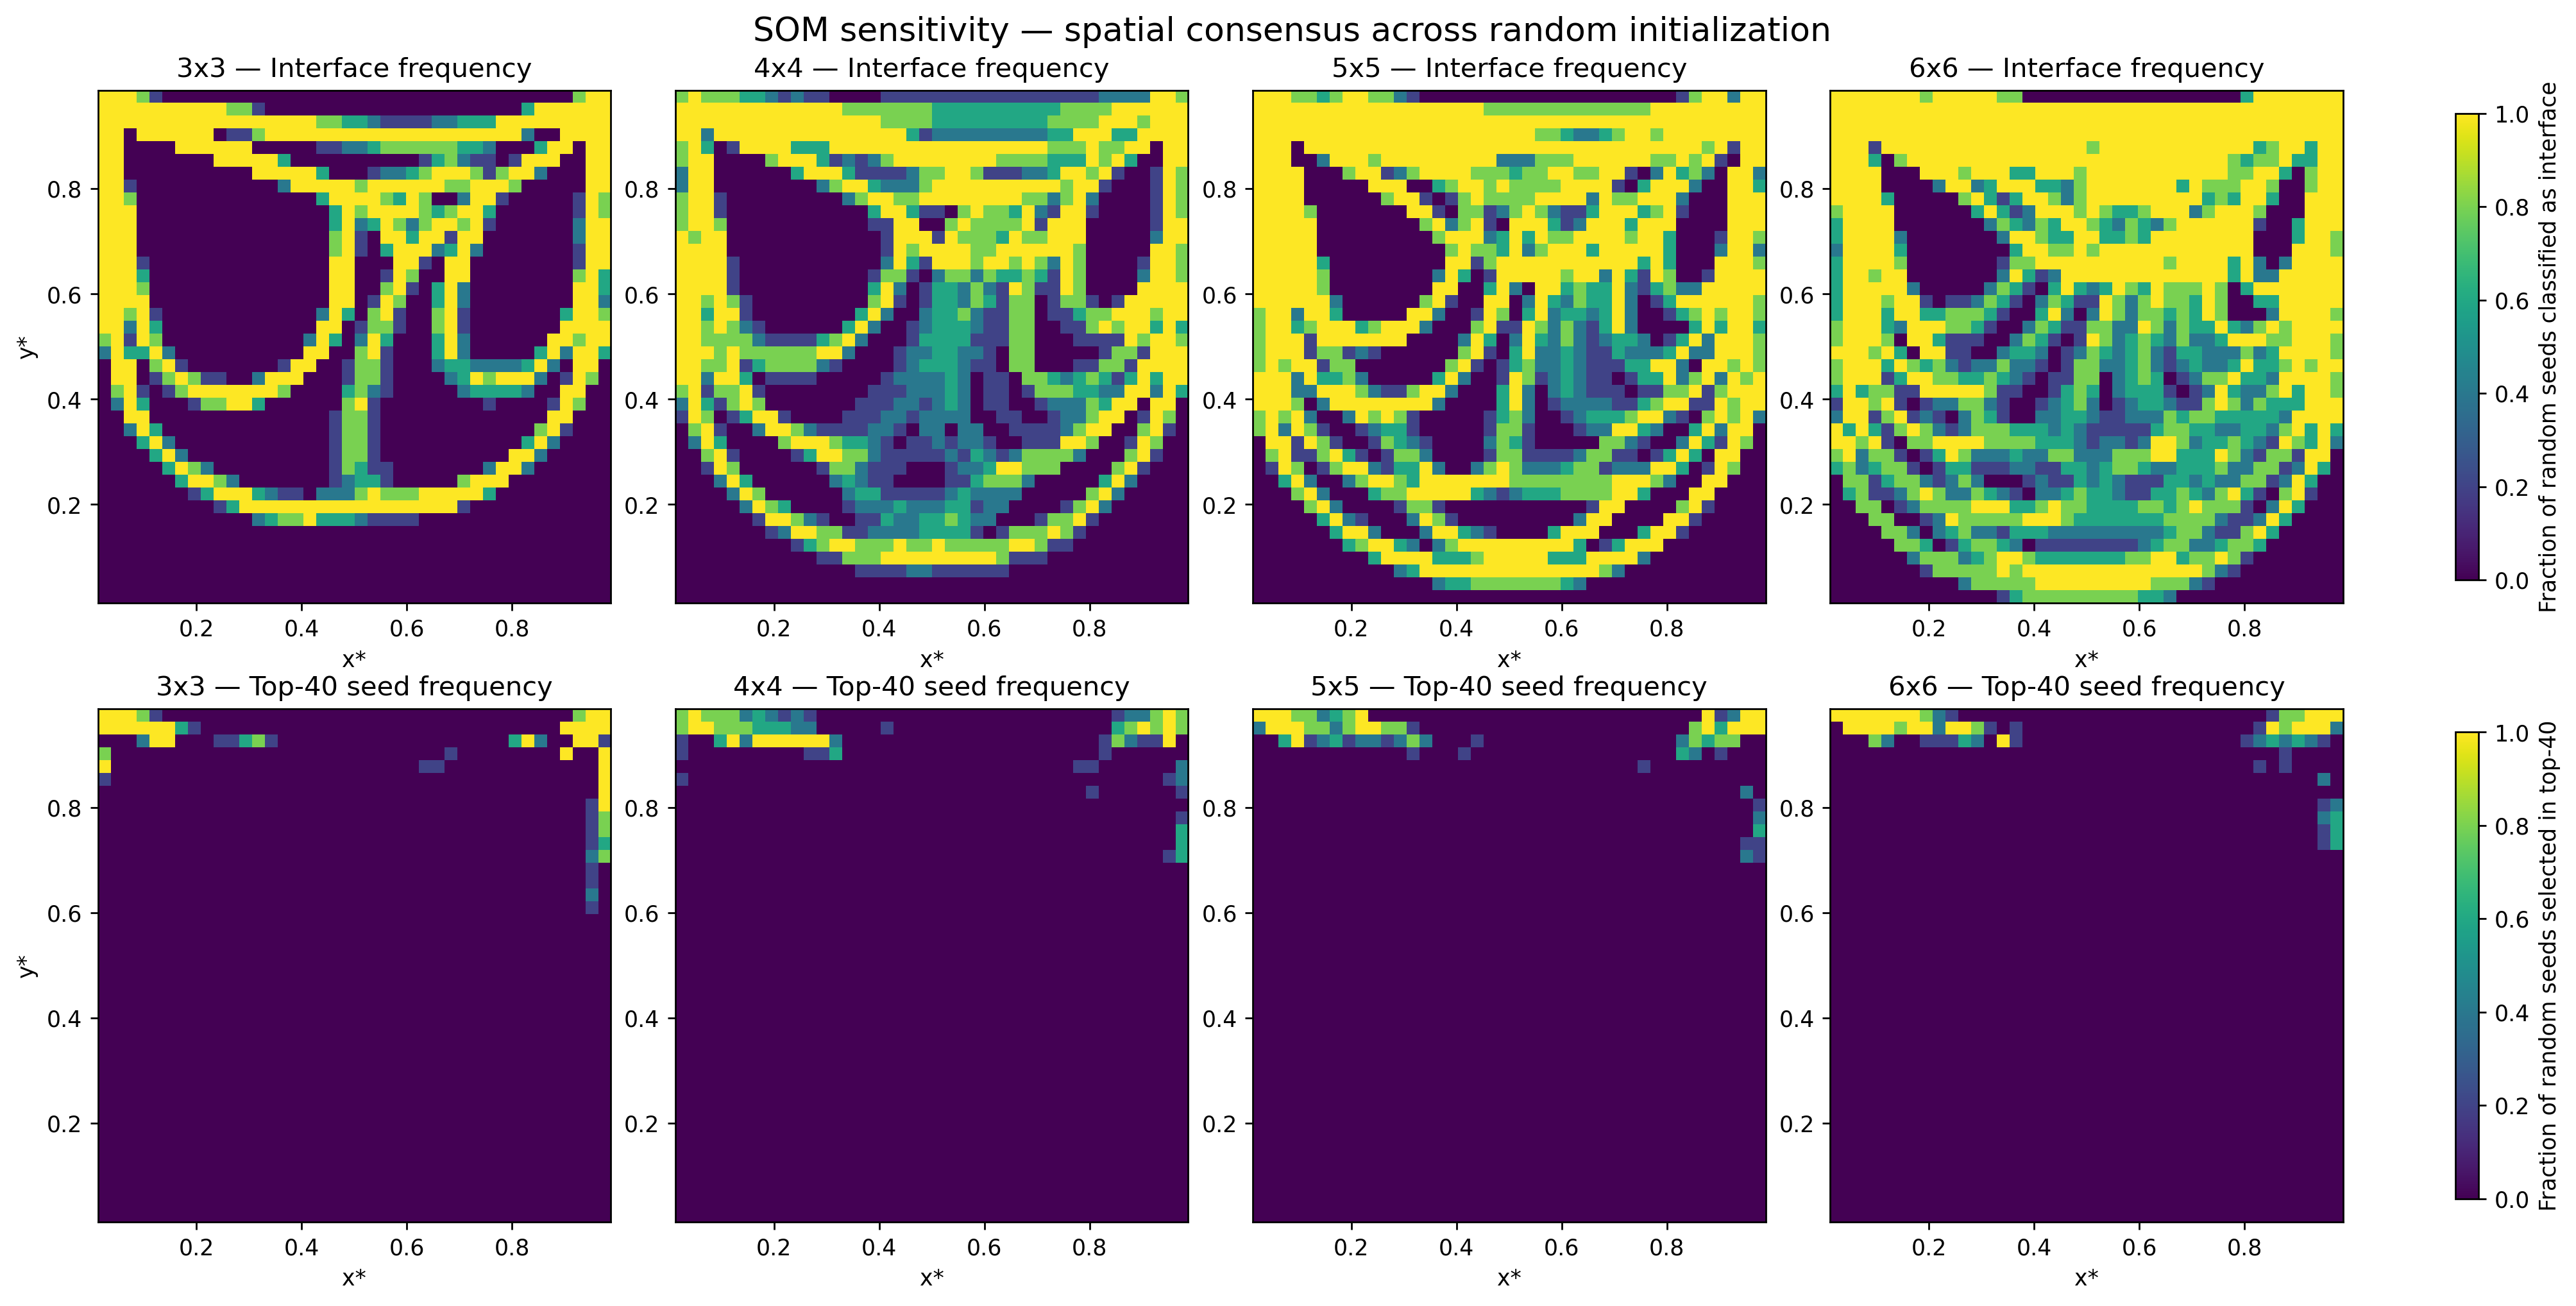
\includegraphics[width=0.98\textwidth]
{figures/som_sensitivity_consensus.png}
\caption{Spatial consensus across five random initializations for the
\(3\times3\), \(4\times4\), \(5\times5\), and \(6\times6\) SOM
architectures. The upper row shows SOM-interface frequency and the lower row
shows Top-40 seed-selection frequency.}
\label{fig:som_sensitivity_consensus}
\end{figure}

The consensus maps reinforce the quantitative results. Increasing the SOM
size produces a denser network of state interfaces, while the highest-priority
interface selections remain concentrated within comparatively localized
regions of the cavity. Differences between random initializations therefore
affect the exact partition and exact selected cells without necessarily
relocating all high-priority selections to unrelated physical regions.

The sensitivity study does not identify a uniquely optimal SOM architecture.
The \(3\times3\) map provides the highest partition stability but the
coarsest representation among the tested configurations. Conversely, the
\(6\times6\) map provides the lowest mean quantization error but generates
the densest interface network and exhibits the lowest mean partition
stability. The \(4\times4\) configuration used in the main adaptive study
should therefore be interpreted as the nominal architecture investigated in
that study, rather than as an architecture demonstrated to be optimal.

More generally, the results demonstrate that SOM architecture and random
initialization constitute relevant modeling choices for the proposed
interface-based refinement framework. Robustness of a fixed-seed result
should not be conflated with robustness to alternative initializations, and
future applications should evaluate architecture and initialization
sensitivity for the flow problem under consideration.


\subsection{Refinement-utility analysis}

To investigate whether the observed differences could be related to the
utility of the selected regions, the adaptive-mesh discrepancy fields were
interpolated back onto the original M40 cell centers. The M40--M160
discrepancy was used only as an evaluation quantity. Cells were partitioned
into four mutually exclusive groups: selected by both methods,
Gradient-only, SOM-only, and selected by neither method.

For the \(1N\) comparison, the mean M40 discrepancy in the common region was
\(2.91\times10^{-2}\). The corresponding post-refinement errors were
\(7.43\times10^{-3}\) for Gradient and \(1.05\times10^{-2}\) for
SOM-interface. In the Gradient-only region, the post-refinement errors were
\(3.60\times10^{-3}\) and \(6.31\times10^{-3}\), respectively. In the
SOM-only region they were \(4.55\times10^{-3}\) and \(4.91\times10^{-3}\).

For the \(2N\) comparison, the common region had a mean M40 discrepancy of
\(2.34\times10^{-2}\), with post-refinement errors of
\(6.44\times10^{-3}\) for Gradient and \(7.25\times10^{-3}\) for
SOM-interface. In the SOM-only region, however, SOM-interface produced a
lower mean post-refinement error than Gradient,
\(3.50\times10^{-3}\) versus \(3.84\times10^{-3}\).

The same analysis also shows that the benefit of either refinement strategy
is not confined to the cells explicitly selected for refinement. In the
regions selected by neither method, SOM-interface produced lower mean
post-refinement error than Gradient in both matched cases. This is
consistent with the globally coupled nature of the CFD solution and
reinforces the need to evaluate refinement strategies through the resulting
solution rather than through local indicator values alone.

\begin{table}[htbp]
\centering
\caption{Spatial refinement-utility analysis for the cell-matched
comparisons. ``SOM better fraction'' is the fraction of M40 locations in
each region for which the interpolated SOM-interface discrepancy is lower
than the corresponding Gradient discrepancy.}
\label{tab:refinement_utility_interface}
\small
\begin{tabular}{llrrrr}
\toprule
Case & Region & \(N\) & M40 error & Gradient error & SOM error \\
\midrule
1N & Both & 53 & 2.907e-2 & 7.434e-3 & 1.053e-2 \\
1N & Gradient-only & 25 & 1.058e-2 & 3.603e-3 & 6.306e-3 \\
1N & SOM-only & 25 & 1.032e-2 & 4.546e-3 & 4.910e-3 \\
1N & Neither & 1497 & 2.205e-3 & 1.523e-3 & 1.145e-3 \\
\midrule
2N & Both & 74 & 2.341e-2 & 6.445e-3 & 7.245e-3 \\
2N & Gradient-only & 40 & 5.936e-3 & 2.551e-3 & 2.940e-3 \\
2N & SOM-only & 40 & 9.194e-3 & 3.844e-3 & 3.496e-3 \\
2N & Neither & 1446 & 2.093e-3 & 1.332e-3 & 9.861e-4 \\
\bottomrule
\end{tabular}
\end{table}

The utility analysis should not be interpreted as a cell-level proof that
SOM-interface is universally superior. Rather, it provides evidence that
the new criterion changes the spatial distribution of refinement in a way
that can produce a different global solution response. In particular, the
\(2N\) case shows a lower error in the SOM-only region, while the common and
Gradient-only regions still favor Gradient on average.


\subsection{Final adaptive-mesh topology}

The differences between the refinement indicators can also be examined
directly through the final computational meshes. Figure~\ref{fig:adaptive_meshes}
compares the SOM-QE and Gradient meshes at the 10\% refinement budget.
Both simulations contain exactly 2080 cells and passed the OpenFOAM mesh
quality checks.

\begin{figure}[htbp]
\centering
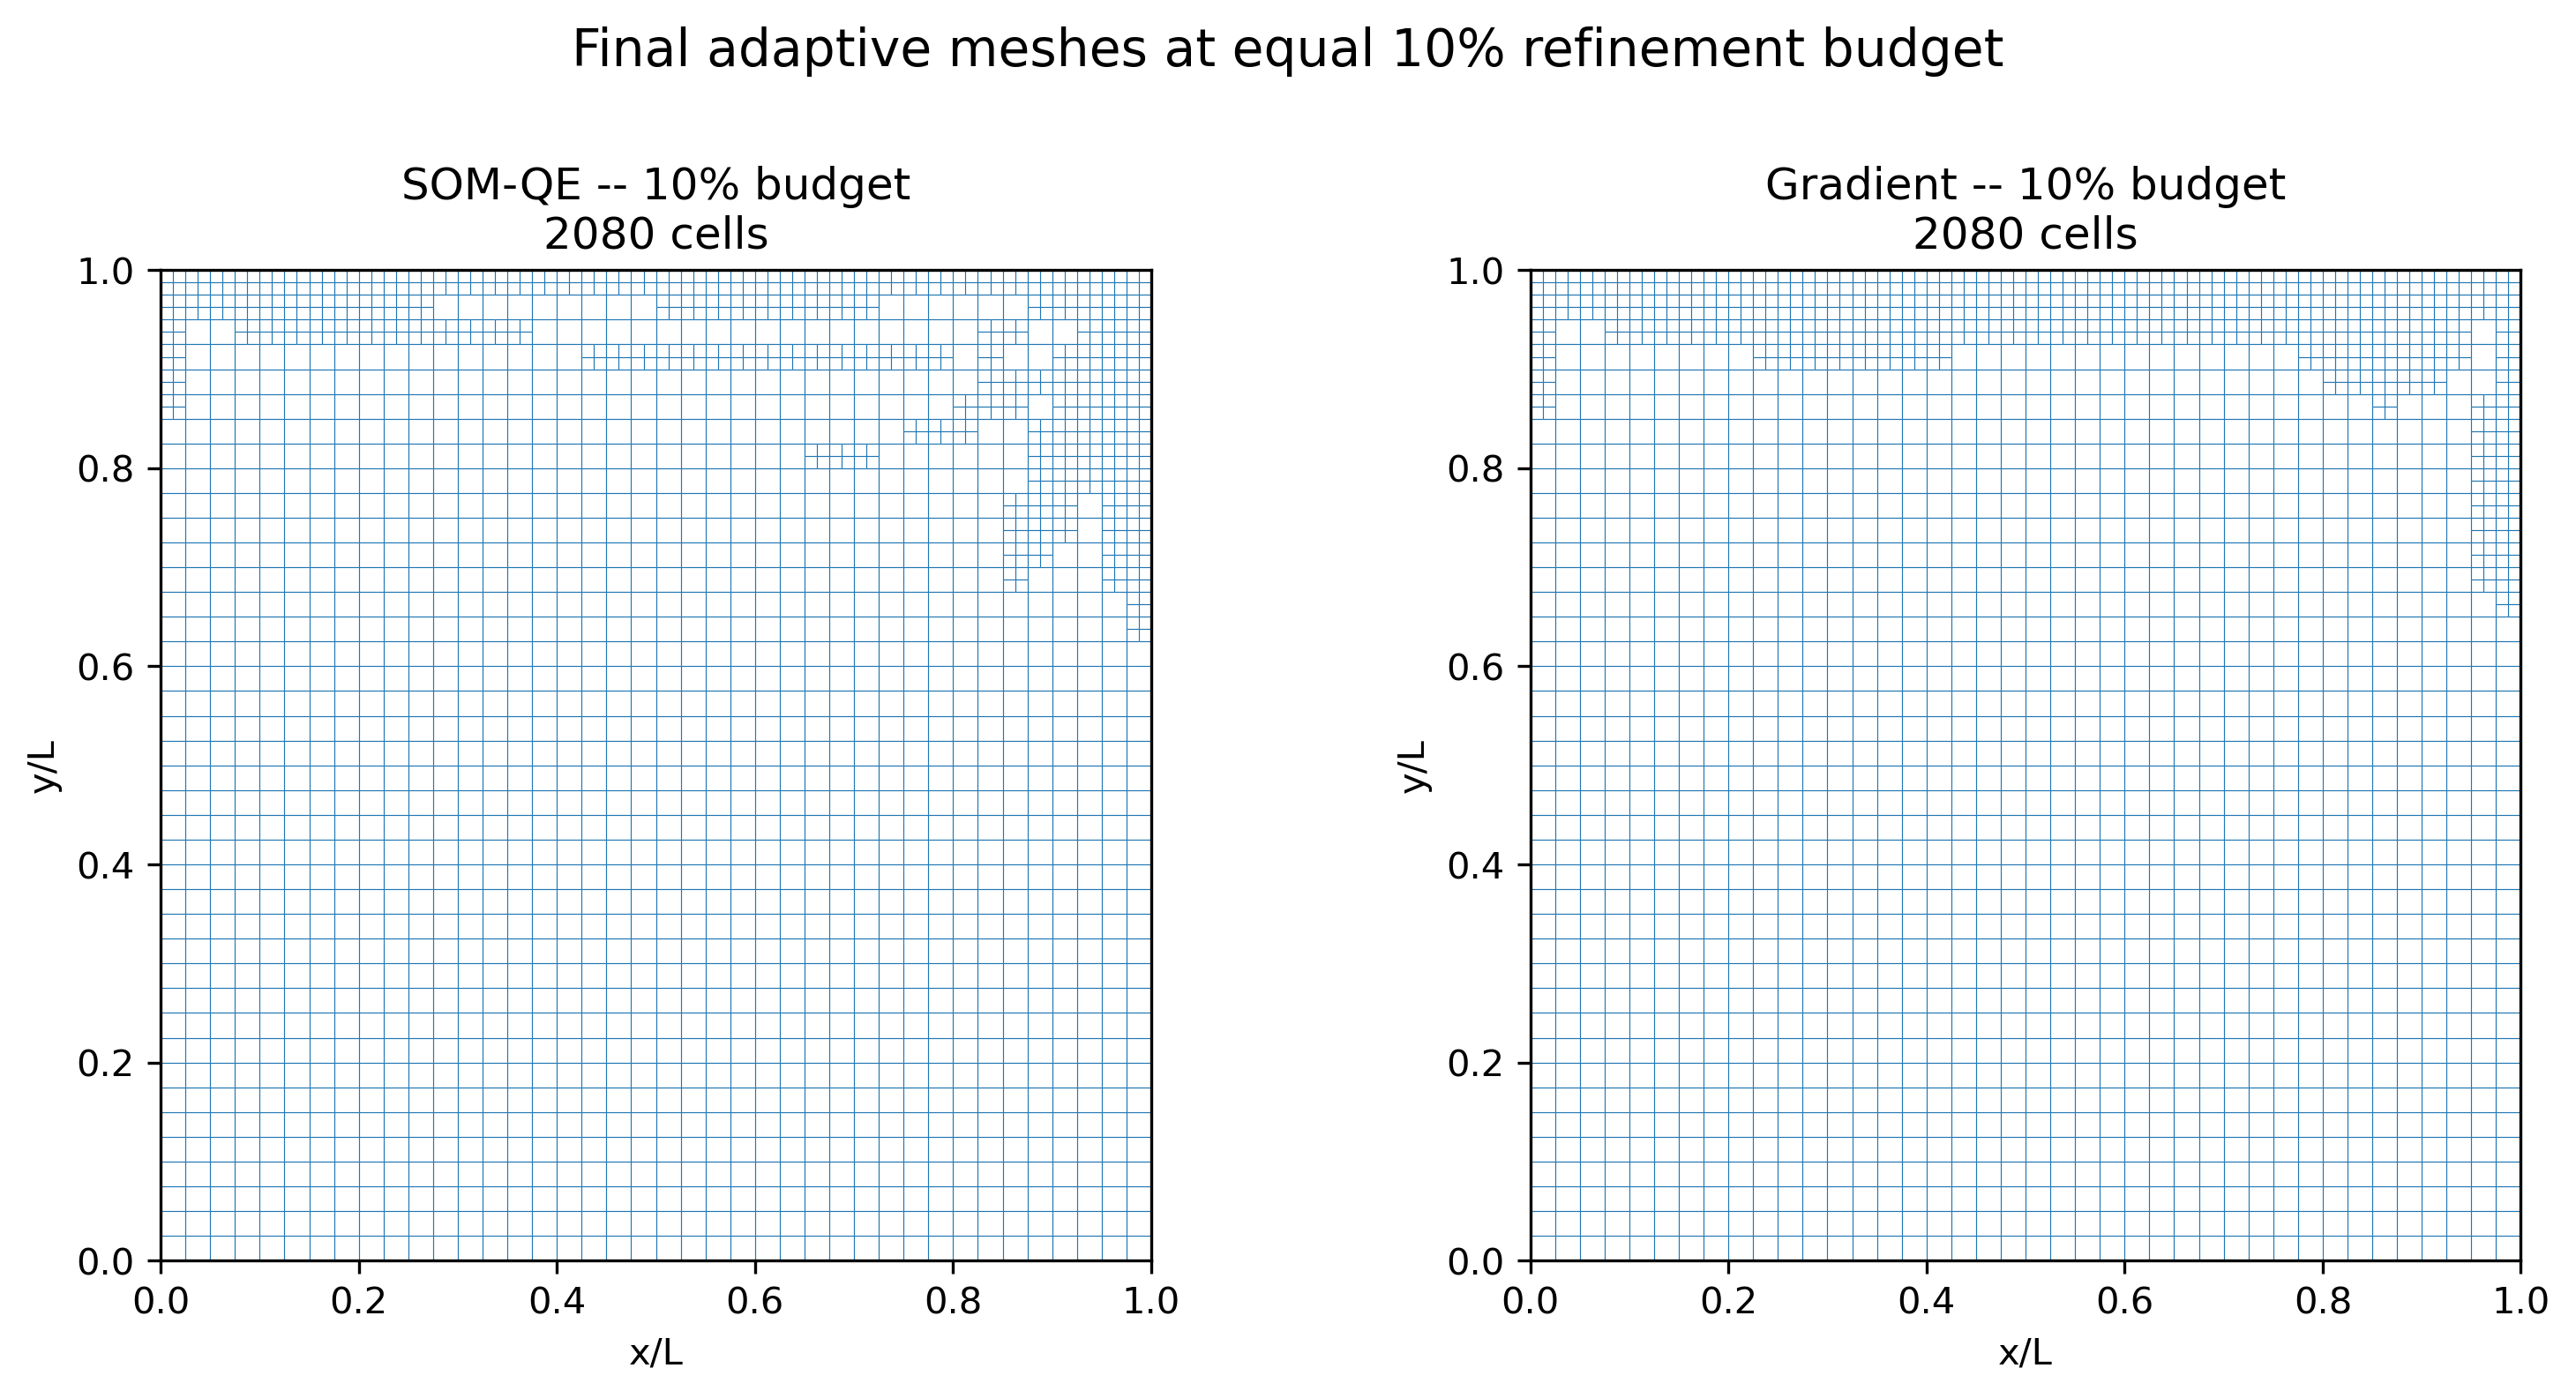
\includegraphics[width=0.98\textwidth]
{figures/Adaptive_mesh_SOM_vs_Gradient_10.png}
\caption{Final adaptive meshes obtained with SOM-QE and Gradient refinement
at the same 10\% refinement budget. Both meshes contain 2080 cells. The
comparison therefore isolates differences in the spatial allocation of
refinement rather than differences in total cell count.}
\label{fig:adaptive_meshes}
\end{figure}

The two indicators allocate the identical refinement budget differently.
Gradient concentrates refinement predominantly near the moving lid and the
upper cavity, where large velocity gradients occur. SOM-QE also refines the
upper region but distributes part of its refinement budget into additional
flow regions extending farther into the cavity.

This distinction is important because the adaptive-mesh comparison shows
that equal numbers of cells do not imply equal numerical performance.
At the 10\% budget, the Gradient mesh produces a lower RMS discrepancy
relative to the M160 reference despite having exactly the same number of
cells as the SOM-QE mesh. The result therefore points to the spatial
allocation of refinement, rather than cell count alone, as the relevant
difference between the two strategies.

